% To je predloga za poročila o domačih nalogah pri predmetih, katerih
% nosilec je Blaž Zupan. Seveda lahko tudi dodaš kakšen nov, zanimiv
% in uporaben element, ki ga v tej predlogi (še) ni. Več o LaTeX-u izveš na
% spletu, na primer na http://tobi.oetiker.ch/lshort/lshort.pdf.
%
% To predlogo lahko spremeniš v PDF dokument s pomočjo programa
% pdflatex, ki je del standardne instalacije LaTeX programov.

\documentclass[a4paper,11pt]{article}
\usepackage{a4wide}
\usepackage{fullpage}
\usepackage[utf8x]{inputenc}
\usepackage[slovene]{babel}
\selectlanguage{slovene}
\usepackage[toc,page]{appendix}
\usepackage[pdftex]{graphicx} % za slike
\usepackage{setspace}
\usepackage{color}
\definecolor{light-gray}{gray}{0.95}
\usepackage{listings} % za vključevanje kode
\usepackage{hyperref}
\usepackage{float}
\usepackage{verbatim}
\renewcommand{\baselinestretch}{1.2} % za boljšo berljivost večji razmak
\renewcommand{\appendixpagename}{Priloge}

\lstset{ % nastavitve za izpis kode, sem lahko tudi kaj dodaš/spremeniš
language=Python,
basicstyle=\footnotesize,
basicstyle=\ttfamily\footnotesize\setstretch{1},
backgroundcolor=\color{light-gray},
}

\title{Tretja domača naloga}
\author{Anže Pečar (63060257)}
\date{\today}

\begin{document}

\maketitle

\section{Uvod}

Cilj domače naloge je bil oddati napovedi na tekmovalni stržnik in se seznaniti z ocenjevanjem točnosti in napovedni modeli.

\section{Metode}
\subsection{Ocenjevanje točnosti}
Ocenjevanje točnosti na učnih podatkih, F mera
\subsection{Napovedni modeli}
\begin{itemize}
\item[1R] V knjigi[bla] sem naletel na preprost algoritem imenovan 1R, ki sem ga nekoliko predelanega uporabil v domači nalogi. Algoritem deluje tako, da za vsak atribut posebej prešteje kolikokrat atribut določa posamezen razred. Napovedovanje na testnih podatkih izgleda tako, da glede na atribute, ki imajo vrednosti večje od 0, dobim seznam najbolj pogostih razredov, ki jih ti atributi napovedujejo. 
\item[RF] Random Forest sem si zgeneriral za 10, 50, 250 in 500 dreves. Razlika med rezultatom za RF z 250 drevesi in 500 so minimalne, se pa 250 kar obnese veliko bolje kot 50. V prvem tednu sem za izbiro napovedanih razredov uporabil samo THRESHOLD vrednost (0.20 se je najbolje obnesla), v drugem tednu pa sem eksperimentiral z različnimi funkcijami. Preprosta izboljšava je bila, da sem dobljene napovedane vrednosti normaliziral preden sem nastavil prag. Še boljša pa je bila implementacija z dinamičnimim pragom, s katero sem dosegel najvišji rezultat.
\end{itemize}
\section{Rezultati}
Moje ime v tekmovalnem sistemu: Anže Pečar
\subsection{Rezultati oddaj}
\begin{table}[H]
\caption{Oddaje}
\begin{tabular}{ c c c c c l }
 Pred 12.3 & Ime metode & Oddaja & ocena mere F & ocena mere F na strežniku & Komentar\\
  \hline
  * & 1R & 12 & 0.36 & 0.36 & Najboljši rezultat metode \\
  \* & RF & 1 & 1 & 1 & Najboljši rezultat metode \\
 \end{tabular}
\end{table}
%\begin{figure}[H]
%\begin{center}
%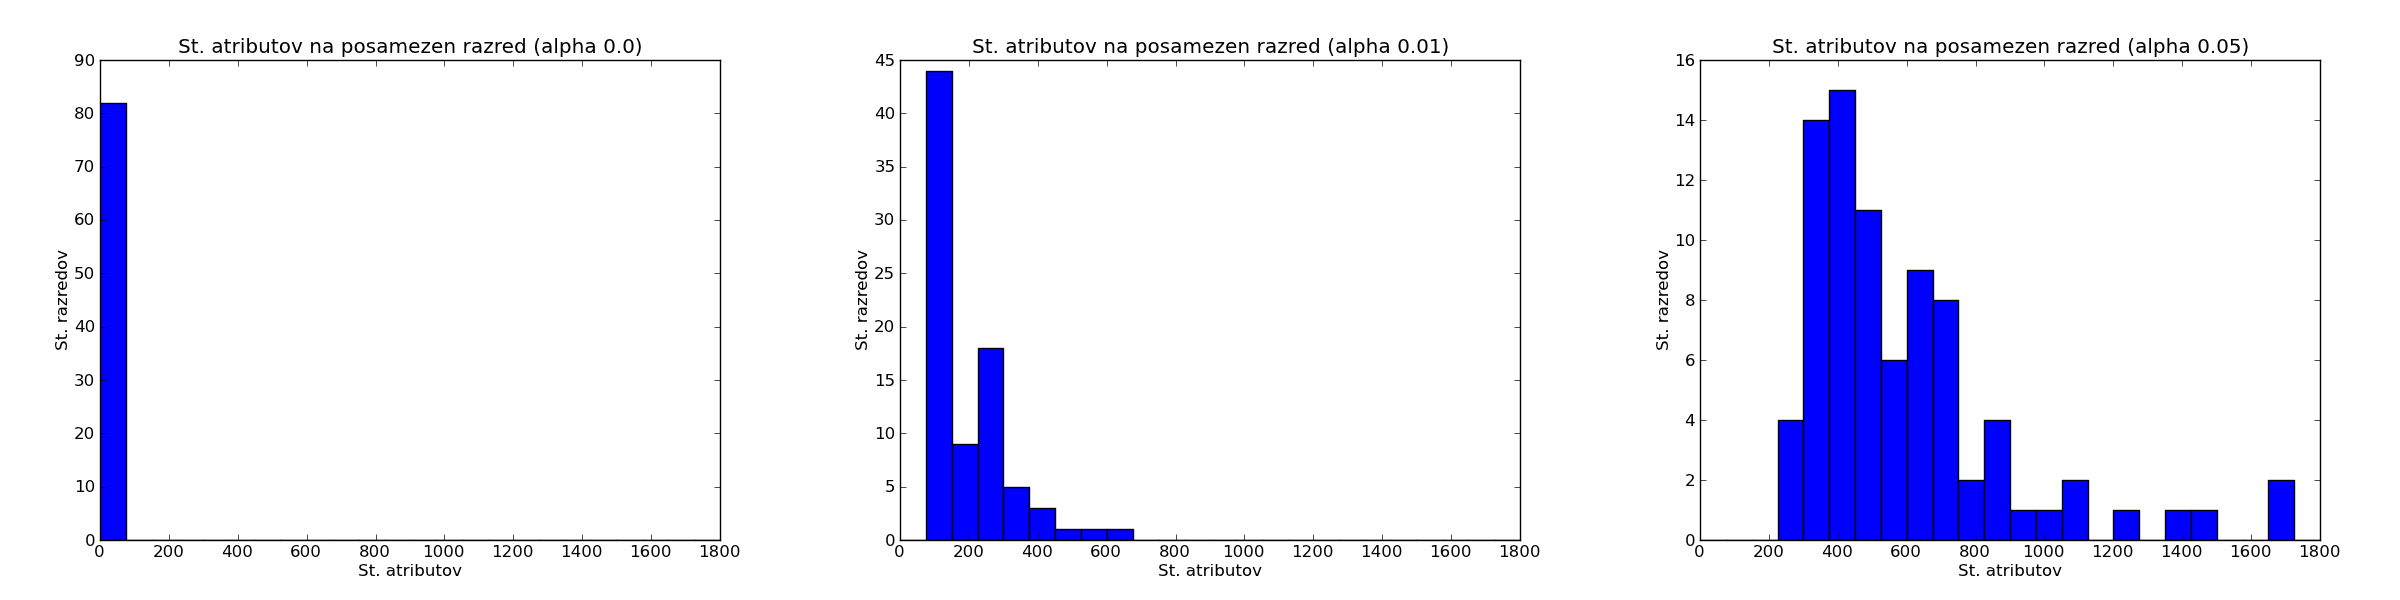
\includegraphics[scale=0.2]{skupno100.png}
%\caption{Rezultati 100 permutacij za različne vrednosti Alpha}
%\label{skupno100}
%\end{center}
%\end{figure}

\subsection{Hitrost izvajanja}
500 RF:
\begin{verbatim}
real	889m59.265s
user	883m40.190s
sys	3m9.084s
\end{verbatim}

\section{Izjava o izdelavi domače naloge}
Domačo nalogo in pripadajoče programe sem izdelal sam.
\end{document}
